\documentclass[12pt, letterpaper]{article}
\usepackage[utf8]{inputenc}
\usepackage{graphicx}
\usepackage{bigints}
\usepackage{tabularx}
\usepackage{caption}
\usepackage{subcaption}
\usepackage{hyperref}
\usepackage{float}

\hypersetup{
    colorlinks=true,
    linkcolor=blue,
    filecolor=magenta,      
    urlcolor=cyan,
}

\graphicspath{ {images/} } 

\title{\textbf{Spaceflight Dynamics}\\
		\large{End Term Report}\\
 		\large{Summer of Science $2020$}}
\author{Nishant Mittal - $190070038$\\
Mentor - Abhishek Raghuvanshi}
\date{June 8, 2020}

\begin{document}
\setlength{\parindent}{0pt}
\maketitle

\begin{figure}[h]
	\centering
    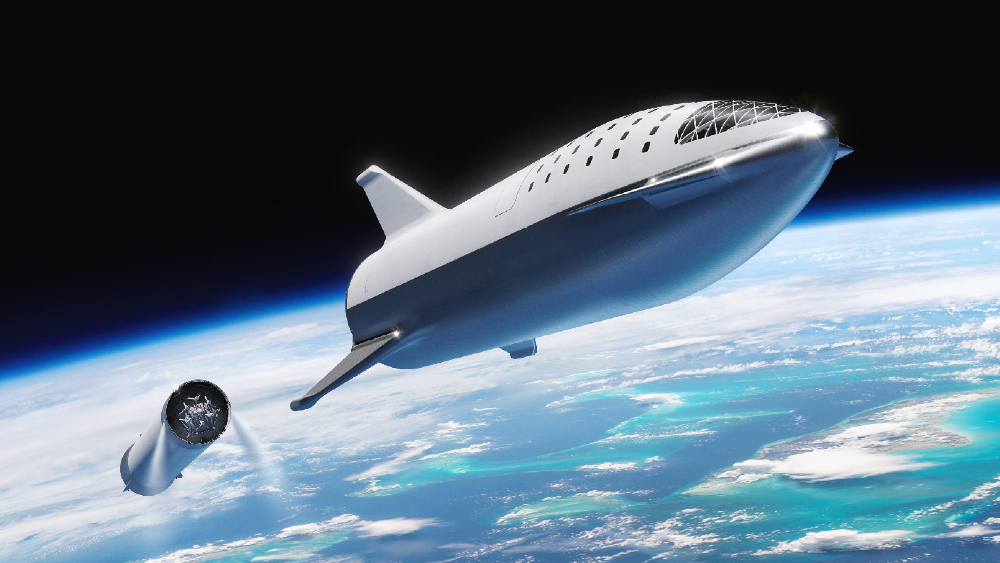
\includegraphics[width=370px]{cover}
\end{figure}

\begin{abstract}
Spaceflight Dynamics is the science of spacecraft performance, stability and control. It involves the modelling of the changing position and orientation of a vehicle and analysis of the effect of various forces on it. In this report, I hope to build a groundwork for the same and explore briefly a few subsets of it. This report shall also strive to explain some other concepts and considerations to keep in mind when thinking about a spacecraft.
\end{abstract}

\newpage
\tableofcontents

\newpage
\section{Introduction - Setting up the Groundwork}
\subsection{Particle Dynamics}
To understand the dynamics of a spacecraft, we must first set up the basis of our study and lay down the basic tools we shall be using to understand and analyse more complex problems. It all starts with Newton's Three Laws:
\begin{enumerate}

	\item A particle at rest remains in rest, and a particle in motion remains in motion, if the applied force is zero.
	\item The force on a particle equals the mass of the particle times its inertial acceleration.
	\item For every force applied, there is an equal and opposite reaction force.

\end{enumerate}

I need not go into the details and explanation of these, we all know their implications, nuances and caveats. Another important set of laws in our analysis are the ones laid down by Keppler. They are as follows:
\begin{enumerate}

	\item The orbit of a planet is an ellipse with the Sun at one of the two foci.
	\item A line segment joining a planet and the Sun sweeps out equal areas during equal intervals of time.
	\item The square of the orbital period of a planet is directly proportional to the cube of the semi-major axis of its orbit.

\end{enumerate}

 These laws were written down by Keppler after detail study and observation of our solar system, hence they describe the motion of planets in our solar system. However these are applicable to a much more general case of the Two Body Problem. We shall see the same in that section. I shall now focus on building upon the math involved in applying these laws when in frames other than the inertial frame.

For starters, let us define the frame $i$ as the inertial frame and $s$ as the non-inertial frame. Now a vector $\mathbf{A}$ can be expressed in the inertial frame as:

\begin{displaymath} \mathbf{A^i} = A_{i1}i_1 + A_{i2}i_2 + A_{i3}i_3 \end{displaymath}
 
 where $i_1, i_2, i_3$ are a set of orthogonal basis vectors of the inertial frame. $\mathbf{A}$ can be represented in 
 the non - inertial frame as:

\begin{displaymath} \mathbf{A^s} = A_{s1}s_1 + A_{s2}i_2 + A_{s3}i_3 \end{displaymath}

where $s_1, s_2, s_3$ are a set of orthogonal basis vectors of the non-inertial frame. These two expressions are just representations of a vector in two different frames of reference, but the vector itself exists independent of any frame. The coordinate $A_i$ and $A_s$ are simply representations of the same vector. Both are related via a rotation matrix as given below. 

\begin{displaymath}
	\begin{bmatrix} A_{i1} \\ A_{i2} \\ A_{i3} \end{bmatrix} 
	=
	\begin{bmatrix}
	i_{1} \cdot s_{1} & i_{1} \cdot s_{2} & i_{1} \cdot s_{3}\\
	i_{2} \cdot s_{1} & i_{2} \cdot s_{2} & i_{2} \cdot s_{3}\\
	i_{3} \cdot s_{1} & i_{3} \cdot s_{2} & i_{3} \cdot s_{3}\\
	\end{bmatrix}
	\cdot
	\begin{bmatrix}
	A_{s1} \\ A_{s2} \\ A_{s3}
	\end{bmatrix}
\end{displaymath}
\begin{displaymath}	\mathbf{A^i} = R^{si}\mathbf{A^s} \end{displaymath}

Suppose the $\mathbf{A}$ vector represents distance. To calculate velocity and acceleration we must differentiate above equation. 

\begin{displaymath}
\frac{d}{dt}\mathbf{A^i} = \frac{d}{dt}(R^{si}\mathbf{A^s}) = \Dot{A^{si}}\mathbf{A^s} + R^{si}\Dot{\mathbf{A^s}}
\end{displaymath}

The rotation matrix when multiplied with its inverse or transpose, disaperars. So we are left with:

\begin{displaymath}
\frac{{}^id}{dt}\mathbf{A} = \frac{{}^id}{dt}\mathbf{A} + R^{siT}\Dot{R^{si}}\mathbf{A^s}
\end{displaymath}

Now suppose the non-inertial frame is rotating with respect to the inertial frame with angular velocity $\mathbf{\omega^{si}}$. It can be shown that $R^{siT}\Dot{R^{si}} = \mathbf{\omega^{si}}$. As $\mathbf{A}$ can be any vector we can say that: 

\begin{displaymath}
\frac{{}^id}{dt}( ) = \frac{{}^id}{dt}( ) + \mathbf{\omega^{si}}\times()
\end{displaymath}

Similarly for acceleration, we must differentiate again. This gives us the following result:

\begin{displaymath}
\frac{{}^id^2}{dt^2}(\mathbf{R + r}) = \frac{{}^id^2}{dt^2}\mathbf{R} + \frac{{}^sd^2}{dt^2}\mathbf{r} + 2\mathbf{\omega^{si}}\times\frac{{}^sd}{dt}(\textbf{r}) + (\frac{{}^sd}{dt}\mathbf{\omega^{si}})\times\mathbf{r} + \mathbf{\omega^{si}}\times(\mathbf{\omega^{si}}\times\mathbf{r})
\end{displaymath}
Where $\mathbf{R}$ is the distance of the origin non-inertial frame from the origin of the inertial frame. What we have established so far along with a few high-school concepts shall make up our toolkit. Until now we have treated mass as dimensionless point particles, which is not the case in reality! We shall now see dynamics of systems if we consider the physical dimensions of the same.

\subsection{Rigid Body Dynamics}

A rigid body is generally a system with six degrees of freedom. Three degrees are related to the translational motion and the other three with rotational motion of the system. 

\subsubsection{Translational Dynamics}

On each particle in the system there will be internal and external forces acting upon it. Applying Newton's second law to each particle in system and summing over all particles, we get:
\begin{displaymath}
\sum \mathbf{F_i} = \sum \mathbf{f_{int}} + \sum \mathbf{f_{ext}} = \sum m_i\mathbf{a_1}
\end{displaymath}


As the internal forces are equal and opposite in nature, the summation of internal forces over the entire system will amount to zero. We shall now define a new term called center of mass and its location $\mathbf{r_{cm}}$ is given as:
\begin{displaymath}
\mathbf{r_{cm}} = \frac{1}{M}\sum_{}^{} m_{i} \mathbf{r_{i}}
\end{displaymath}
 Combining the two equations we get:

 \begin{displaymath}
 \mathbf{F_e} = \sum \mathbf{f_{ext}} = \frac{d^2}{dt^2}\mathbf{r_{cm}}
 \end{displaymath}

This implies the center of mass behaves as if all the mass of the rigid body was concentrated there and all the external force was applied there.This covers the translational degrees of freedom. Note in the above formulation, if the system is a made up of a continuous particle system, the summation is converted to an integral and $m_i$ to $dm$. Now to tackle the rotational degrees of freedom.

\subsubsection{Rotational Dynamics}

To analyse rotational dynamics, we must first encounter a quantity known as angular momentum($\mathbf{H}$). It is defined as follows:
\begin{displaymath}
\mathbf{H} = \int \mathbf{r} \times \mathbf{\omega} dm 
\end{displaymath}
Taking a reference frame tied to the body we get:
\begin{displaymath}
\mathbf{H} = \int \mathbf{r} \times (\mathbf{\omega^{bi}} \times \mathbf{r}) dm 
\end{displaymath}

where $\mathbf{\omega^{bi}}$ is the inertial angular velocity of the rigid body. We are now in a body frame of reference. Through splitting the terms into their components and further calculations we get:

\begin{displaymath}
\mathbf{H} = \bigintsss
	\begin{bmatrix}
	y^2 + z^2 & -yz &  -zx\\
	 -xy &  z^2 + x^2 &  -zy\\
	 -xy & -yz & x^2 + y^2\\
	\end{bmatrix}
	dm
	\begin{bmatrix}
	\omega_1\\
	\omega_2\\
	\omega_3\\
	\end{bmatrix}
\end{displaymath}

Here we define a new quantity called moment of inertia(I) given as:

\begin{displaymath}
	I = 
	\begin{bmatrix}
	\int(y^2 + z^2)dm & \int(-yz)dm & \int(-zx)dm\\
	\int(-xy)dm & \int(z^2 + x^2)dm & \int(-zy)dm\\
	\int(-xy)dm & \int(-yz)dm & \int(x^2 + y^2)dm\\
	\end{bmatrix}
\end{displaymath}

This gives us:

\begin{displaymath}
\mathbf{H} = I \mathbf{\omega^{bi}}
\end{displaymath}

Here \textbf{H} is not parallel to the angular velocity vector. This is not desirable. Thus we focus on a particular body frame called the principal axis frame. In this frame the moment of inertia tensor can be represented as a diagonal matrix. This frame can always be found by diagonalising the moment of inertia matrix via solving its characteristic equation. We now move onto relating this with torque(\textbf{M}). Torque is generally given as:
\begin{displaymath}
\mathbf{M} = \frac{{}^id}{dt}\mathbf{H}
\end{displaymath}

Substituting the above equation for angular momentum and doing further calculations we get:

\begin{displaymath}
\mathbf{M} = I\dot{\mathbf{\omega^{bi}}} + \mathbf{\omega^{bi}}\times I \mathbf{\omega^{bi}}
\end{displaymath}

These give three non-linear first order differential equations make up half of the equations required to fully describe the rotational motion of a system. To obtain the second half of the dynamics it is necessary to introduce three angles specifying the orientation of the body with respect to the inertial frame and relate them to $\mathbf{\omega^{bi}}$. We shall do so using the classical euler angles: pitch, roll and yaw.

\begin{figure}[h]
	\centering
    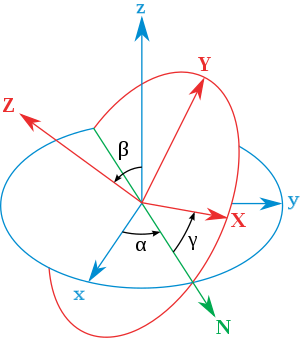
\includegraphics[width = 200px]{EulerAngles}
    \caption{Euler's Angles}
\end{figure}

The Euler angles $\phi,\theta,\psi$ are shown in figure 1. The inertial frame is shown in blue while the body frame is in red. One goes from inertial frame to body frame by first rotating along the '\textbf{z}' axis by $\phi$ then about the node vector \textbf{N} by $\theta$ and finally about '\textbf{Z}' by $\psi$. The total rotation can be written as:

\begin{displaymath}
R^{ib} = R_3^{T}(\psi)R_1^{T}(\theta)R_1^{T}(\phi)
\end{displaymath}

Where $R_1$ and $R_3$ are elementary rotation matrices about the x and z axes respectively. Now from the figure we can write $\omega^{bi}$ as:

\begin{displaymath}
\mathbf{\omega^{bi}} = \dot{\phi}\mathbf{i_1} + \dot{\theta}\mathbf{n} + \dot{\psi}\mathbf{b_1}
\end{displaymath}

Upon further simplification, we can write $\omega^{bi}$ in its body frame components as:

\begin{gather*}
\omega_1 = \dot{\phi}sin{\theta}sin{\psi} + \dot{\theta}cos\psi\\
\omega_2 = \dot{\phi}sin{\theta}cos{\psi} - \dot{\theta}sin\psi\\
\omega_3 = \dot{\psi} + \dot{\phi}cos\theta
\end{gather*}

Also, via the differentiation rule and using the rotation matrix defined above, we can also get:

\begin{displaymath}
\dot{\mathbf{b_i}} = \mathbf{\omega^{bi}}\times\mathbf{b_i}
\end{displaymath}

These complete the necessary equations required to completely analyse the rotational motion of a system. There are other techniques such as \href{https://en.wikipedia.org/wiki/Quaternion}{quaternion rotation} that are alternatives to Euler's angles that are advantageous in certain case scenarios. \href{https://quaternions.online}{Here} is an online tool that shows the relation between quaternions and Euler's Angles. Given this we are now ready to start further analysis of more complex systems. We shall start with the famous two body problem.

\newpage
\section{The Two Body Problem}
 The two body problem is the simplest gravitational problem, just two point masses orbiting under their mutual gravitational attraction. The problem is to describe the motion of both objects given initial conditions. Let there be two masses with distances from a inertial origin as shown in Figure 2.

\begin{figure}[h]
	\centering
    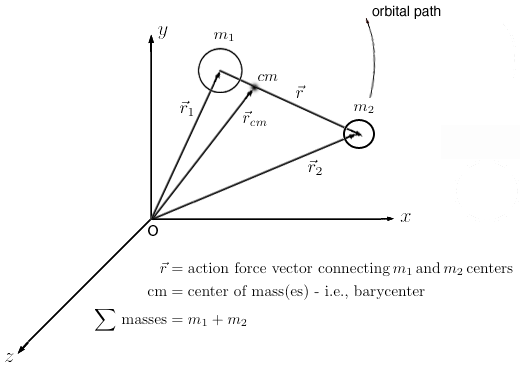
\includegraphics[width = 300px]{Twobodies}
    \caption{Two particles as seen from inertial frame}
\end{figure}

By equating gravitational forces on each object:
\begin{gather*}
m_1\mathbf{\ddot{R}_{1}} = \frac{-Gm_1m_2}{|\mathbf{R_2} - \mathbf{R_1}|^3}(\mathbf{R_1} - \mathbf{R_2})\\
m_2\mathbf{\ddot{R}_{2}} = \frac{-Gm_1m_2}{|\mathbf{R_2} - \mathbf{R_1}|^3}(\mathbf{R_2} - \mathbf{R_1})\\
\end{gather*}

Adding, we get:
\begin{displaymath}
m_1\mathbf{\ddot{R}_{1}}  + m_2\mathbf{\ddot{R}_{2}} = 0
\end{displaymath}

We also introduce another vector $\mathbf{R_{cm}}$ given as:
\begin{gather*}
\mathbf{R_{cm}} = \frac{m_1\mathbf{R_1}+m_2\mathbf{R_2}}{m_1 + m_2}
\end{gather*}
Hence, we get:
\begin{gather*}
\mathbf{\ddot{R}_{cm}} = 0 \\
\mathbf{R_{cm}} = \mathbf{R_{cm0}} + \mathbf{V_{cm0}}t
\end{gather*}

Where $\mathbf{R_{cm0}}$ and $\mathbf{V_{cm0}}$ are the position and velocity vectors of the center of mass at $t=0$ and are constants. From Figure 2, $\mathbf{r} = \mathbf{R_2} - \mathbf{R_1}$ is obvious. By using the initial force equations, we can see:

\begin{displaymath}
m_1m_2 \mathbf{\ddot{r}} = \frac{-Gm_1m_2(m_1+m_2)}{r^3}\mathbf{r}
\end{displaymath}

Writing $\mu = G(m_1+m_2)$, we get:
\begin{displaymath}
\mathbf{\ddot{r}}  = \frac{-\mu\mathbf{r}}{r^3}
\end{displaymath}

This equation describes relative motion. Taking dot product of above equation with $\mathbf{\dot{r}}$ and further simplification, we get:

\begin{gather*}
\begin{split}
\frac{d}{dt}\frac{1}{2}\dot{r}^2 & = - \frac{\mu}{r^2}\dot{r}\\
								& = - \frac{d}{dt}\left(-\frac{\mu}{r}\right)
\end{split}
\end{gather*}

Substituting,
\begin{displaymath}
V = -\frac{\mu}{r}
\end{displaymath}

Where V is the potential energy per unit mass, we get:
\begin{displaymath}
\mathcal{E} = \frac{1}{2}v^2 + V
\end{displaymath}

Hence the total energy is conserved. Note, here $\mathcal{E}$ represents the total energy per unit mass and not the entire mechanical energy. This is beneficial in some case scenarios and can be easier to work with. We shall now attempt to find the orbit equation. To do this, take cross product with radius vector $\mathbf{r}$ on both sides of relative motion equation. The R.H.S goes to zero as cross product of vector with itself is zero. Integrating we get:

\begin{displaymath}
\mathbf{r}\times\mathbf{\dot{r}} = \mathbf{H}
\end{displaymath}

Here \textbf{H} is the angular momentum per unit mass which is again a constant. Here \textbf{H} is also equal to twice the rate of description of the position vector of $m_2$ with respect to $m_1$. This proves Keppler's second law. Now to solve the initial differential equation, take right hand cross product of relative motion equation with \textbf{H}. Upon solving further, we get:

\begin{displaymath}
\mathbf{r} = \frac{\mathbf{H^2}/\mu}{1 + e\:cos\nu}
\end{displaymath}

Where $\mathbf{e}$ is a integration constant vector. It is termed as the \textit{eccentricity vector} and its scalar magnitude is simply the eccentricity of the orbit while direction is from the focus to the perigee of the orbit. The angle $\nu$ is the angle between the position vector($\mathbf{r}$) and the eccentricity vector and is termed as the \textit{true anomaly}. The above equation is the polar form of a conic section with the origin as one of the focii. If $e < 1$, the orbit is elliptical, $e = 1$ implies a parabolic orbit and $e > 1$ implies a hyperbolic orbit. We shall see in depth analysis of these in a later section. Now, the two body problem was completely solvable and we got a neat result. But real life has certainly more than just two bodies. Let us now look into the N Body Problem.

\subsection{The N Body Problem}

We shall start by employing a route similar to that of the two body problem. Define $ \mathbf{r_{ij}} = \mathbf{R_{j}} - \mathbf{R_{i}}$. Applying Gravitational Law on each object:

\begin{displaymath}
m_i\mathbf{\ddot{r}_i} = \sum_{j \neq i}^{N} \frac{Gm_im_j}{r_{ij}^3}\mathbf{r_{ij}}
\end{displaymath}

When we sum all the above equations, the R.H.S goes to zero due to Newton's third law. All forces are equal and opposite and cancel each other out in the summation. We get:

\begin{displaymath}
\sum_{i=1}^{N} m_i\mathbf{\ddot{r}_i} = 0
\end{displaymath}

This leads us to:

\begin{gather*}
M\mathbf{\ddot{r}_{cm}} = 0\\
\mathbf{r_{cm}}(t) = \mathbf{r_{cm0}} + \mathbf{V_{cm0}}t
\end{gather*}

Following the steps taken in the two body problems with a few minor modifications, we can obtain the following quantities:

\begin{gather*}
\mathbf{H} = \sum_{i=1}^{N} m_i\mathbf{r_i}\times\mathbf{\dot{r}_i}\\
V = -\frac{1}{2}\sum_{i=1}^{N}\sum_{j \neq i}^{N}\frac{Gm_im_j}{r_{ij}}\\
\mathcal{E} = \sum_{i=1}^{N}\frac{1}{2}m_i\mathbf{\dot{r}_i}\cdot\mathbf{\dot{r}_i} + V
\end{gather*}

This all we can absolutely determine for a N-Body system. Further solutions cannot be obtained "absolutely" and through various mathematical techniques and approximations, we can obtain models that nearly replicate real life systems. In the next section let's dive a bit deeper into the study of orbits.

\newpage

\section{More About Orbits}
As seen in the previous section, the shape of the orbit largely depends on the value of the eccentricity vector. We shall now see the different shapes the orbits take on for different values of eccentricity as well as how the other physical quantities are limited and dependent by the orbit shape.
\subsection{Conical Orbits}

Conical orbits are simply the orbits that are obtained from slicing a cone at different angles with a plane. There are five resulting shapes namely: the circle, ellipse, parabola, hyperbola, and the straight line. The last is simply free fall and occurs when an object is simply dropped with no initial horizontal velocity hence it isn't a orbit per se. A circular orbit is perhaps the simplest orbit, occurring when $e=0$, it has uniform distance from the second object and uniform speed across its entire motion. Hence we shall not be discussing those two shapes here. Let us start from a bounded orbit.

\subsubsection{Elliptical Orbit}

This orbit is seen for cases when $e<1$. 

\begin{figure}[ht]
	\centering
    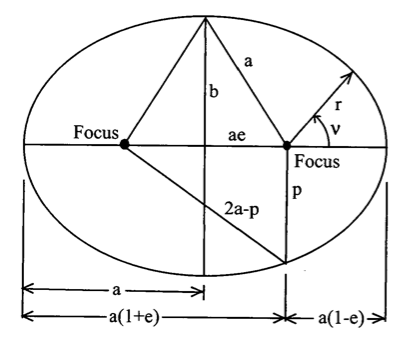
\includegraphics[width = 200px]{ellipse}
    \label{fig:ellipse}
    \caption{Elliptical Orbit}
\end{figure}

To begin, let's write out the ellipse relation: $b = a\sqrt{1-e^2}$. If we set $\nu = 90^\circ$, we get $p = H^2/\mu$. By Pythagoras theorem, we get:
\[
	(2ae)^2 + p^2 = (2a -p)^2
\] 
This simplifies to:
\[p=a(1-e^2)\]
This also gives us:
\[H = \sqrt{\mu p} = \sqrt{\mu a(1-e^2)}\]

Note here perigee occurs at $\nu = 0^\circ$. Hence the eccentric vector is towards the right. Now as we have angular momentum, we can calculate the speed of the object at any point on the orbit. At the perigee, the velocity vector and position vector are perpendicular to each other. Hence:
\begin{gather*}
	\mathbf{H} = \mathbf{r\times v}\\
	\implies H_p = r_pv_p\\
	\implies v_p = \frac{\sqrt{\mu a(1-e^2)}}{r_p}
\end{gather*}

Using that in the energy relation, we get:
\begin{gather*}
\begin{split}
	\mathcal{E} &= \frac{1}{2}v_p^2 - \frac{\mu}{r_p}\\
	&= - \frac{\mu}{2a}
\end{split}
\end{gather*}

Thus, we finally get:
\[ v^2  = \mu \left(\frac{2}{r} - \frac{1}{a}\right) \]
As the range of $r$ is from $r_p = a(1-e)$ to $r_a = a(1+e)$, we get the range of $v$ as $v_a = \sqrt{\frac{\mu}{a}\left(\frac{1-e}{1+e}\right)} $ to $v_p =  \sqrt{\frac{\mu}{a}\left(\frac{1+e}{1-e}\right)} $. If we put $e=0$, we get the velocity required for a circular orbit as:

\[ v_c = \sqrt{\frac{\mu}{a}} \]
\newpage
\subsubsection{Parabolic Orbit}
This orbit is seen for cases when $e=1$. 

\begin{figure}[ht]
	\centering
    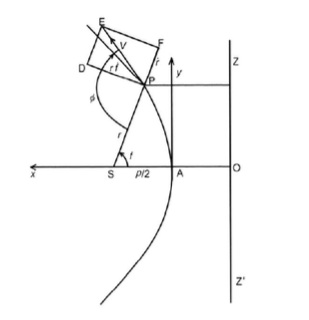
\includegraphics[width = 200px]{parabola}
    \label{fig:parabola}
    \caption{Parabolic Orbit}
\end{figure}
We start by writing orbit equation:
\[ r = \frac{H^2/\mu}{1+cos\nu} \]
Solving at perigee:
\begin{gather*}
	a = \frac{H^2/\mu}{1+cos0^\circ}\\
	\implies H = \sqrt{2\mu a}
\end{gather*}

As per previous working, this gives us:
\[ v = \sqrt{\frac{2\mu}{r}} \]

Hence if the velocity of release at perigee is $\sqrt{\frac{2\mu}{a}}$ the trajectory will be parabolic. Note that the velocity of the object at infinity is zero, hence this is also the minimum velocity with which the object must travel to escape the gravitational field of the other object. This is termed as escape velocity. Note that $v_e = \sqrt{2}v_c$.
\newpage
\subsubsection{Hyperbolic Orbit}
This orbit is seen for cases when $e>1$. 
\begin{figure}[ht]
	\centering
    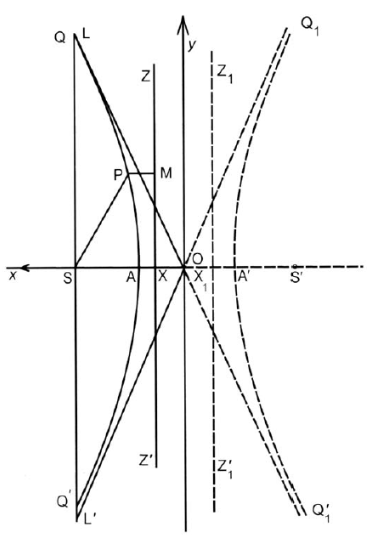
\includegraphics[width = 200px]{hyperbola}
    \label{fig:hyperbola}
    \caption{Hyperbolic Orbit}
\end{figure}

Again, working along the same lines as the previous orbits:
\[ r = \frac{H^2/\mu}{1+e\:cos\nu} \]
Solving at perigee:
\begin{gather*}
	a(e-1) = \frac{H^2/\mu}{1+e\:cos0^\circ}\\
	\implies H = \sqrt{\mu a(1-e^2)}
\end{gather*}
Relating with energy equation, we get similar results. The thing to be noted here is the non-zero velocity the object has as  it reaches infinity. This is called residual velocity and is given by:
\[ 
	v_\infty = \sqrt{\frac{\mu}{a}}
\]

If we got back to the orbit equation keeping in mind that $e>1$ we will see another notable fact. There is a maximum angle to which the object can go and the orbit is bounded by asymptotes as also seen in Figure 5. It is given by:
\[
	\nu_\infty = cos^{-1}\left( \frac{-1}{e} \right)
\]

This \href{https://evgenii.com/blog/two-body-problem-simulator/}{link} is a simulator for the two body problem. By varying eccentricity and mass ratio, the different orbits can be observed.

\subsection{Orbital Elements}
There are six parameters which completely define the orbit of an object. These are called orbital elements.

\begin{figure}[ht]
	\centering
    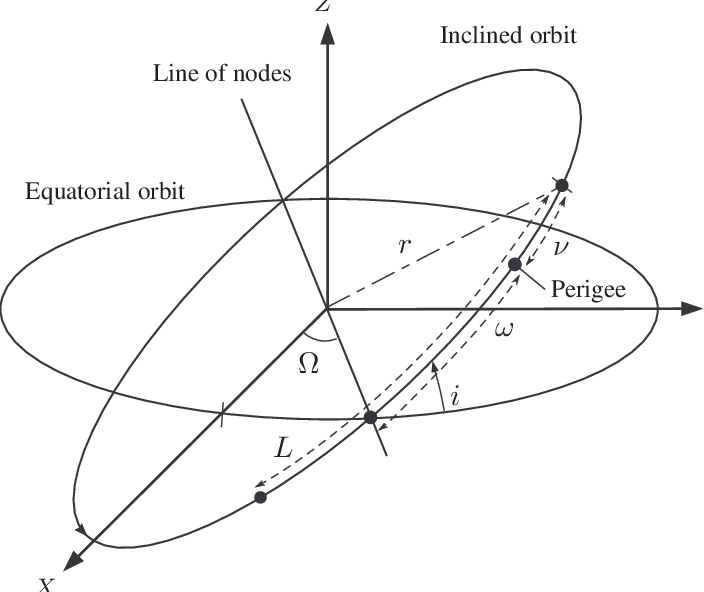
\includegraphics[width = 200px]{orbital_elements}
    \label{fig:elements}
    \caption{Orbital Elements}
\end{figure}
The xy plane is the equatorial plane of the Earth, while the z axis is along the rotation axis of Earth. The x axis is tied to the vernal equinox. This is taken as the base reference with respect to which, six parameters are defined according to Figure 6. The semimajor axis($a$) defines the size of the orbit while the eccentricity($e$) defines the shape of the orbit. Inclination($i$) is used to define the orientation of the orbit with respect to the Earth's equator. Argument of Perigee($\omega$) defines where the low point, or perigee, of the orbit is with respect to the Earth's surface. Right Ascension of the Ascending Node($\Omega$) defines the location of the ascending and descending orbit locations with respect to the Earth's equatorial plane and True/Mean Anomaly($\nu$) defines where the satellite is within the orbit with respect to perigee.

\newpage
\section{Other Considerations}
\subsection{Aerodynamics}
Rocket aerodynamics is the study of how air flows over a rocket and how this affects drag and stability. The nose cone and fins of a rocket are designed to minimise drag and to provide stability and control. The drag equation is given by:
\[
	F_{drag} = -\frac{1}{2}\: \rho \: C_d \: A v^2 \: \hat{\mathbf{v}}
\]

Where $C_d$ is the drag coefficient and depends on the geometry of the rocket(nose and fins influence this), A is the surface area, $\rho$ is the density of the medium in which the craft is travelling and $v$ is the velocity with which the craft is travelling. As is clear from the above equation, drag force is negligible beyond the exosphere where there is very low density of particles. An important concept in rocket stability is the center of pressure. It is the average point where which the force of the net pressure field in exerted. What this means for us is the point where the lift and drag forces act. Note that this point may not be(and often isn't) at the same position as the center of mass. For a rocket to be inherently stable the center of pressure must be closer to the tail than the center of mass while ascent. The further the are, the more stable the rocket is without external control systems. The following figures should explain:

\begin{figure}[h!]
\centering
\begin{subfigure}{.5\textwidth}
  \centering
  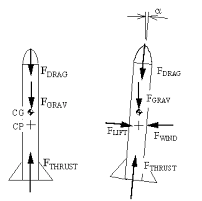
\includegraphics[width=150px]{stable}
  \caption{Stable}
  \label{fig:stable}
\end{subfigure}%
\begin{subfigure}{.5\textwidth}
  \centering
  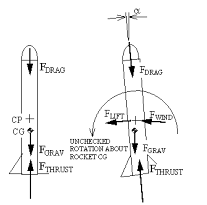
\includegraphics[width=150px]{unstable}
  \caption{Unstable}
  \label{fig:unstable}
\end{subfigure}
\caption{Center of Mass Position influences natural stability}
\label{fig:COP}
\end{figure}

As seen in \ref{fig:unstable}, having the center of pressure above the center of mass produces a torque about the center of mass whenever the rocket tilts over that contributes to the de-stability and produces unchecked rotation. On the other hand, as shown in \ref{fig:stable}, having the center of pressure below the center of mass, the resulting torque is oriented to naturally pull the rocket back to the equilibrium(upright) position. The center of pressure is majorly influenced by the position and size of the tail fins along with the overall shape of the craft. The center of mass is as seen, dependent on the mass distribution along the craft. Beyond the exosphere, these discussions have little consequence, we shall see what does affect crafts in space.

\subsection{A Few Considerations about Space}
So a craft going to space faces a wide variety of problems. We'll discuss two of them here:

\subsubsection{Spacecraft Temperature}
Maintaining the temperature aboard a manned or unmanned spacecraft is crucial to the correct functioning of the craft and survival of its occupants. We know that ideal absorbers are also ideal emitters. We can use this to design radiators that help maintain the temperature of a spacecraft. For ease of working and calculations, we assume our radiators to be ideal. The basic relation we use is the Stephen - Boltzmann Law:
\[
	E(T) = \sigma \:T^4 
\]
This law tells us the total energy emitted by the body at any given temperature. The constant $\sigma$ has a value of $5.672 \: \times \: 10^{-5} $ in cgs units. This law can be used to estimate the equilibrium temperature of a body. Let us take the example of the space shuttle to demonstrate. The space shuttle had flat plate radiators with coolant running behind them with an area of $111\: m^2$.
They were placed underneath the payload bay doors and worked one at a time. Suppose they were exposed to the blackness of space, they would be mainly receiving starlight and the background radiation of about $3K$. Under these conditions:
\[
	E_{out} = \frac{1}{2}\sigma \:T^4 A= 2.55\: \times \: 10^{11} ergs/s \approx 25\:kW
\] 
So the shuttle caries off nearly a heat load of $25\:kW$ when facing empty space. Similar calculations can show that when facing the Earth, the heat load is nearly $6.7\:kW$ and while facing the Sun(which is a perfect blackbody), the shuttle will be forced to absorb nearly $152\:kW$.

\subsubsection{Radiation}

Another problem crafts face in space is of particle radiation. High energy charged particles have devastating effects on the human DNA and have severe biological consequences definitely posing a threat to manned flight, but have troublesome effects on unmanned vehicles as well. On Earth, we are protected by Earth's magnetic field and atmosphere. In space, within the Van Allen belts, there is little protection provided by the magnetic field, but beyond that fatal doses of radiation are a major threat to space exploration. To overcome this, we use shielding and clever positioning of structural components to provide maximum shielding while minimizing weight. However, skimping on material may cause more harm than good, as thin layers can create more radiation via pair production! It is not feasible to shield the entire craft with thick layers to provide protections against solar flares and larger doses of radiation. Hence for long distance journeys, a "storm shelter" has been proposed, which is simply a heavily shielded space where the crew can live for a few days on end. 

As mentioned above, radiation can also cause difficulties with electronic equipments. Most chips are made by doping a perfect crystal lattice of a semiconductor to introduce imperfections. When charged particles travel throughout these lattices, they interact mainly with the imperfections. This can cause many errors within the circuitry. There is also problems of static charge accumulation that can short out and potentially destroy all the circuitry aboard.

\newpage
\section{Inter - Planetary Motion}

The ultimate goal of our work here is to explore new worlds and planets. To do that we must devise an optimal way to get there! Plotting interplanetary trajectories is as simple as solving the N - Body problem but as we have seen before, there is unfortunately no closed solution to the aforementioned problem. Hence we have come up with an approximation technique called \textit{The Sphere of Activity} or the concept of \textit{Patched Conics}. The idea is simple, after a certain distance from any stellar object, the gravitational force asserted by said body is overshadowed by the force of another object, but within that distance, the original object's force dominates. Keeping this in mind, the N - Body problem could be approximated down to different two body problems. When in the sphere of activity of one object, the motion of a spacecraft could be approximated to a two body system. We shall now see a brief proof of the same.

\begin{figure}[ht]
	\centering
    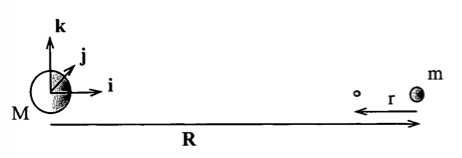
\includegraphics[width = 300px]{ASphere}
    \label{fig:ASphere}
    \caption{Activity Sphere Proof}
\end{figure}

Taking assumptions as in diagram and assuming the test mass to be "in equilibrium", we can write the net inertial acceleration of the test mass between the Earth and the Sun as:
\[
	\mathbf{a_g} = -\frac{GM\mathbf{i}}{(R-r)^2} + \frac{Gm\mathbf{i}}{r^2}
\]

The Earth has an angular velocity of:
\[
	\omega = \left(\frac{GM}{R^3}\right)^{1/2} \: \mathbf{k}
\]
The centripetal acceleration of the mass can be written as:
\begin{equation}
\begin{split}
	\mathbf{a} & = \omega \times(\omega \times (\mathbf{R} - \mathbf{r}))\\
				& = - \frac{GM}{R^3}(R - r)\mathbf{i}
\end{split}
\end{equation}

As the mass is in "equilibrium" i.e. at rest when seen form the rotating frame, equating the centripetal acceleration to the inertial acceleration and applying binomial approximation gives us the following result:

\[
	\frac{r}{R} = \left( \frac{m}{3M} \right)^{1/3}
\]

Now, when this equation is used to calculate the radii of objects in our solar system, it is shown that our earlier approximation holds good for planets and our Sun. Yet the concept of a sphere of activity cannot be applied to systems such as the Earth and its moon. Having this in place we shall now see the concept of Hohmann Transfer.

\subsection{Hohmann Transfer}
Hohmann Transfer is a method devised to transfer from one planetary orbit to another. It is a simple matter of velocity manipulation at the perigee and apogee of an elliptical orbit connecting two circular orbits as shown in the figure below. 

\begin{figure}[h!]
	\centering
    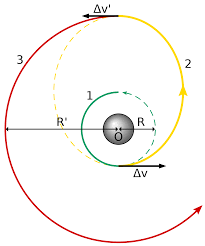
\includegraphics[width = 130px]{Hohmann}
    \label{fig:Hohmann}
    \caption{Hohmann Transfer}
\end{figure}

We've already discussed the underlying concepts and building upon them to derive the necessary increase and decrease in velocity is a trivial matter. Considering $a_t = (R + R')/2$, it can be easily derived that the time taken to transfer from one orbit to another is given by:

\[
	T_{12} = \pi \left(\frac{a_t^3}{\mu}\right)^{1/2}
\]

The Hohmann Transfer fixates on being a method which requires the least amount of energy, the handoff being it requires the greatest amount of time to perform. If we consider the Sun as our center and use a Hohmann Transfer from Earth's orbit to that of Mars, we get a transfer time of about 258 days. At this magnitude of a time frame another problem arises, the time and place at which the craft must be released from Earth's orbit must be planned to intercept Mars when the craft reaches Mars's orbit. This gives motive to look into the concept of Launch Windows.

\subsection{Launch Windows}
\begin{figure}[h!]
	\centering
    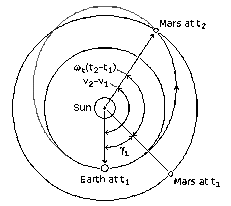
\includegraphics[width = 200px]{Mars}
    \label{fig:Mars}
    \caption{Earth to Mars Transfer}
\end{figure}

There needs to be certain angular relationship between the two planets for the transfer to work. Considering the receiving planet(here Mars) goes on a nearly circular orbit for the duration of the transfer, the relationship can be easily determined as:
\[
	\gamma = \pi - \omega_{t} T_{12}
\]

The time when this relationship is nearly in place is called the Launch Window for the transfer. Taking this into account, around trip journey from Mars is estimated to be about 4 years in total! This is not acceptable. Planetary Flybys' are used to keep the energy requirement at a  low while reducing the time required for deep space missions.

\subsection{Planetary Flyby}

The radius of the activity sphere is considerably larger than that of the planet, hence it is a safe approximation to say that the velocity of the craft at the border of the activity sphere would be similar to that of a hyperbola at $\infty$. I.e. the magnitude of the velocity would be $v_{\infty}$(as derived in earlier sections), and its angle of approach would be equal to $cos^{-1}(-1/e)$. Now whenever we cross the activation sphere, our system shifts from the heliocentric view to the planetary view or vice versa. 

\begin{figure}[h!]
	\centering
    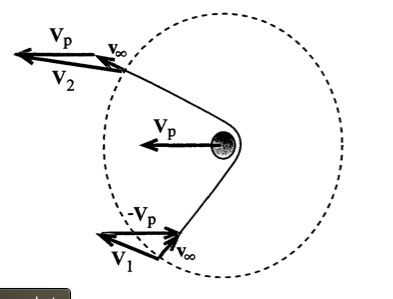
\includegraphics[width = 200px]{Flyby}
    \label{fig:Flyby}
    \caption{How Flybys affect velocity}
\end{figure}

In the figure, $\mathbf{V_p}$ is the velocity of the planet w.r.t the Sun. Similarly, $\mathbf{V_1}$ and $\mathbf{V_2}$ are the velocities of the craft before and after the flyby. Writing the equations:

\[
	\mathbf{v_1 = V_1  - V_p}
\]
\[
	\mathbf{V_2 = v_2  + V_p}
\]

Although $ |\mathbf{v_1}| = |\mathbf{v_2}|  = v_\infty$, the direction of both velocities can differ greatly in terms of both magnitude and direction after the flyby. If the heliocentric velocity is considerably increased after the flyby it is termed as a \textit{trailing side} flyby and \textit{leading side} flyby if the velocity is reduced in magnitude. These both are useful in different cases. If the purpose was simply to change direction, provide speed and head to a different end destination, the trailing side might be preferred. But if the purpose was to perform a scientific flyby, the velocity after the flyby is of little consequence.

\newpage
\section{Rocket Dynamics}
In this section, we shall look at how rockets are actually propelled, a few considerations taken while designing one and the various nuances of the field. 
\subsection{The Rocket Equation}

\begin{figure}[ht]
	\centering
    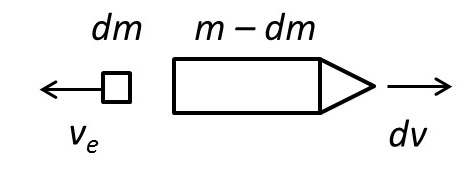
\includegraphics[width = 200px]{rocket_thrust}
    \label{fig:rt}
    \caption{Momentum Conservation}
\end{figure}

The velocity $\mathbf{V_e}$ is relative to to the craft, applying momentum conversation:

\[
	(m + dm)(\mathbf{v} + \mathbf{dv}) -dm(\mathbf{v} + \mathbf{V_e}) = m\mathbf{v}
\]
\[
	md\mathbf{v} -dm\mathbf{V_e} = 0
\]
Divide by $dt$, we get the final equation:
\[
	\mathbf{F_{ext}} + \frac{dm}{dt}\mathbf{V_e} = m\mathbf{a}
\]

This is the rocket equation but is yet incomplete. We assumed the ejected gasses are at the same pressure as the atmosphere. If they are different, there is a correction factor:

\[
	\mathbf{F_{ext}} + \frac{dm}{dt}\mathbf{V_e} - A(P_e - P_a)\mathbf{\hat{V}_e} = m\mathbf{a}
\]
As can be seen clearly from the above equation, the performance would be better within the atmosphere than in outer space. Obviously this is a problem as any rocket spends only a small fraction of its life in the atmosphere. We shall address this problem later on. First, let's define some terms that will help us later on.\\
A rocket's mass is made up of primarily three things: the propellant($m_p$), the body($m_s$) and the payload($m_*$). A payload ratio is defined as:
\[
	\pi = \frac{m_*}{m_0}
\]
And the structural ratio as:
\[
	\epsilon = \frac{m_s}{m_s+_p}
\]
Another quantity called the effective exit velocity is given as:
\[
	V_{e,eff} = V_e - \frac{A}{dm/dt}(P_e - P_a)
\]

Using the newly defined quantities, we can easily integrate our rocket equation. Considering the rocket is in free space with the exhaust pressure dropped to zero, we get:
\[
	v(t) = V_eln\frac{m_0}{m(t)}
\]
The burnout velocity i.e. the velocity of the craft when all the fuel runs out is given by:

\[
	v_b = -V_eln(\epsilon + (1-\epsilon) \pi)
\]

Very clearly, the performance of the rocket depends largely on the structural mass, and hence getting rid of unnecessary weight is crucial for better results. This leads to the concept of multi-stage rockets.

\subsection{Multistage Rockets}
In multistage rockets, initial stages required to provide enough thrust for liftoff are shed when emptied, thereby reducing the amount of parasitic mass. The initial mass of the $k^{th}$ stage($m_{0,k} $) includes the mass of everything above the separation stage for that plane. The final mass of the $k^{th}$ stage($m_{fk} $) is the structural mass of that stage plus the mass of the stages left. Thus definitions are now:

\[
	\epsilon_k = \frac{m_{sk}}{m_{sk} + m_{pk}}
\] 

\[
	\pi_k = \frac{m_{0,k+1}}{m_{0,k}}
\]

With these definitions, each stage can be treated as a single stage rocket. Hence we can apply the previous equation to get the net burnout velocity or the velocity of the payload deployed as:
\[
	V_* = - \sum_{k=1}^{N} V_{ek}ln(\epsilon_k + (1-\epsilon_k) \pi_k)
\]

We now wish to optimize the staging to obtain the greatest payload mass for a given vehicle mass. Note that $V_{ek}$ cannot be mathematically optimized, it is a physical constraint while trying to optimize $\epsilon_{k}$ would yield $0$. The only parameter we can control is $\pi_k$ and it represents the mass distribution amongst the various stages.

\[
	ln\pi_* = \sum_{k=1}^{N} ln\pi_k
\]

This is what we must maximize with the constraint as the earlier equation. We have (N - 1) independent quantities which we can change. We can use the method of Lagrange Multiplier to solve this optimization problem.

\[
	ln\pi_* = \sum_{k=1}^{N}\left( ln\pi_k + \lambda \left\{ \frac{V_*}{N} + V_{ek}ln(\epsilon_k + (1-\epsilon_k) \pi_k) \right\} \right) 
\]

Now calculating the partial derivatives:
\[
	\frac{\partial ln\pi_*}{\partial ln\pi_k} = \frac{1}{\pi_k} + \frac{\lambda V_{ek}(1 - \epsilon_k)}{\epsilon_k + (1-\epsilon_k) \pi_k} = 0
\]

Solving according to the method, we get:

\[
	V_* = - \sum_{k=1}^{N} V_{ek} ln\left( \epsilon_k - \frac{\epsilon_k}{1 + \lambda V_{ek}} \right)
\]
This can be solved via numerical techniques and back substituted to get $\pi_k$ for every k.\\

The multistage rocket also solves the earlier problem of single stages performing better in the atmosphere than in space. 
Another \href{https://www.grc.nasa.gov/WWW/K-12/rocket/rktstage.html}{simulator} to see the effect of staging a rocket.
\newpage
\subsection{The Bell Nozzle}
The bell nozzle takes high energy gas travelng in all directions and streamlines it so the gasses are flowing in one direction.

\begin{figure}[ht]
	\centering
    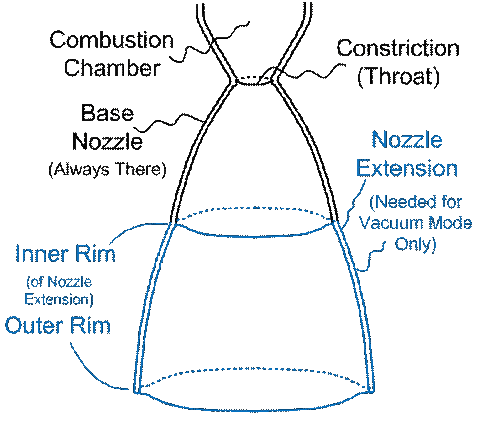
\includegraphics[width = 150px]{nozzle}
    \label{fig:nozzle}
    \caption{The Bell Nozzle}
\end{figure}

The pressure near the constriction of the nozzle is of the order of hundred bars of pressure. As the area of cross section increases, the pressure drops in almost proportion to the area. While traveling in the atmosphere, the pressure required at the end of the nozzle is nearly 1 bar while the nozzle used in space must have the exhaust pressure near zero. As can be seen from the pictures below, the vacuum nozzle is clearly much larger in size than its atmospheric counterpart.

\begin{figure}[ht]
	\centering
    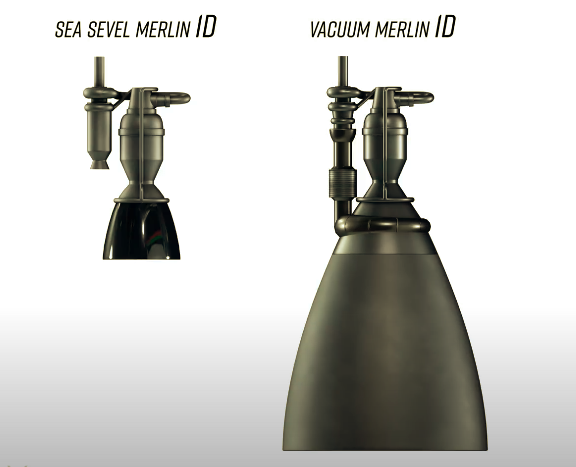
\includegraphics[width = 200px]{comp}
    \label{fig:comp}
    \caption{Size Difference between a Sea Level and a Vacuum Nozzle}
\end{figure}

These are images of Spacex's Merlin engines. A few more on the rocket to give a good idea of how big they actually are:

\begin{figure}[ht]
	\centering
    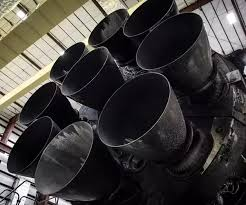
\includegraphics[width = 220px]{nineboosters}
    \label{fig:nineboosters}
    \caption{Nine Sea Level Engines on First Stage}
\end{figure}

\begin{figure}[ht]
	\centering
    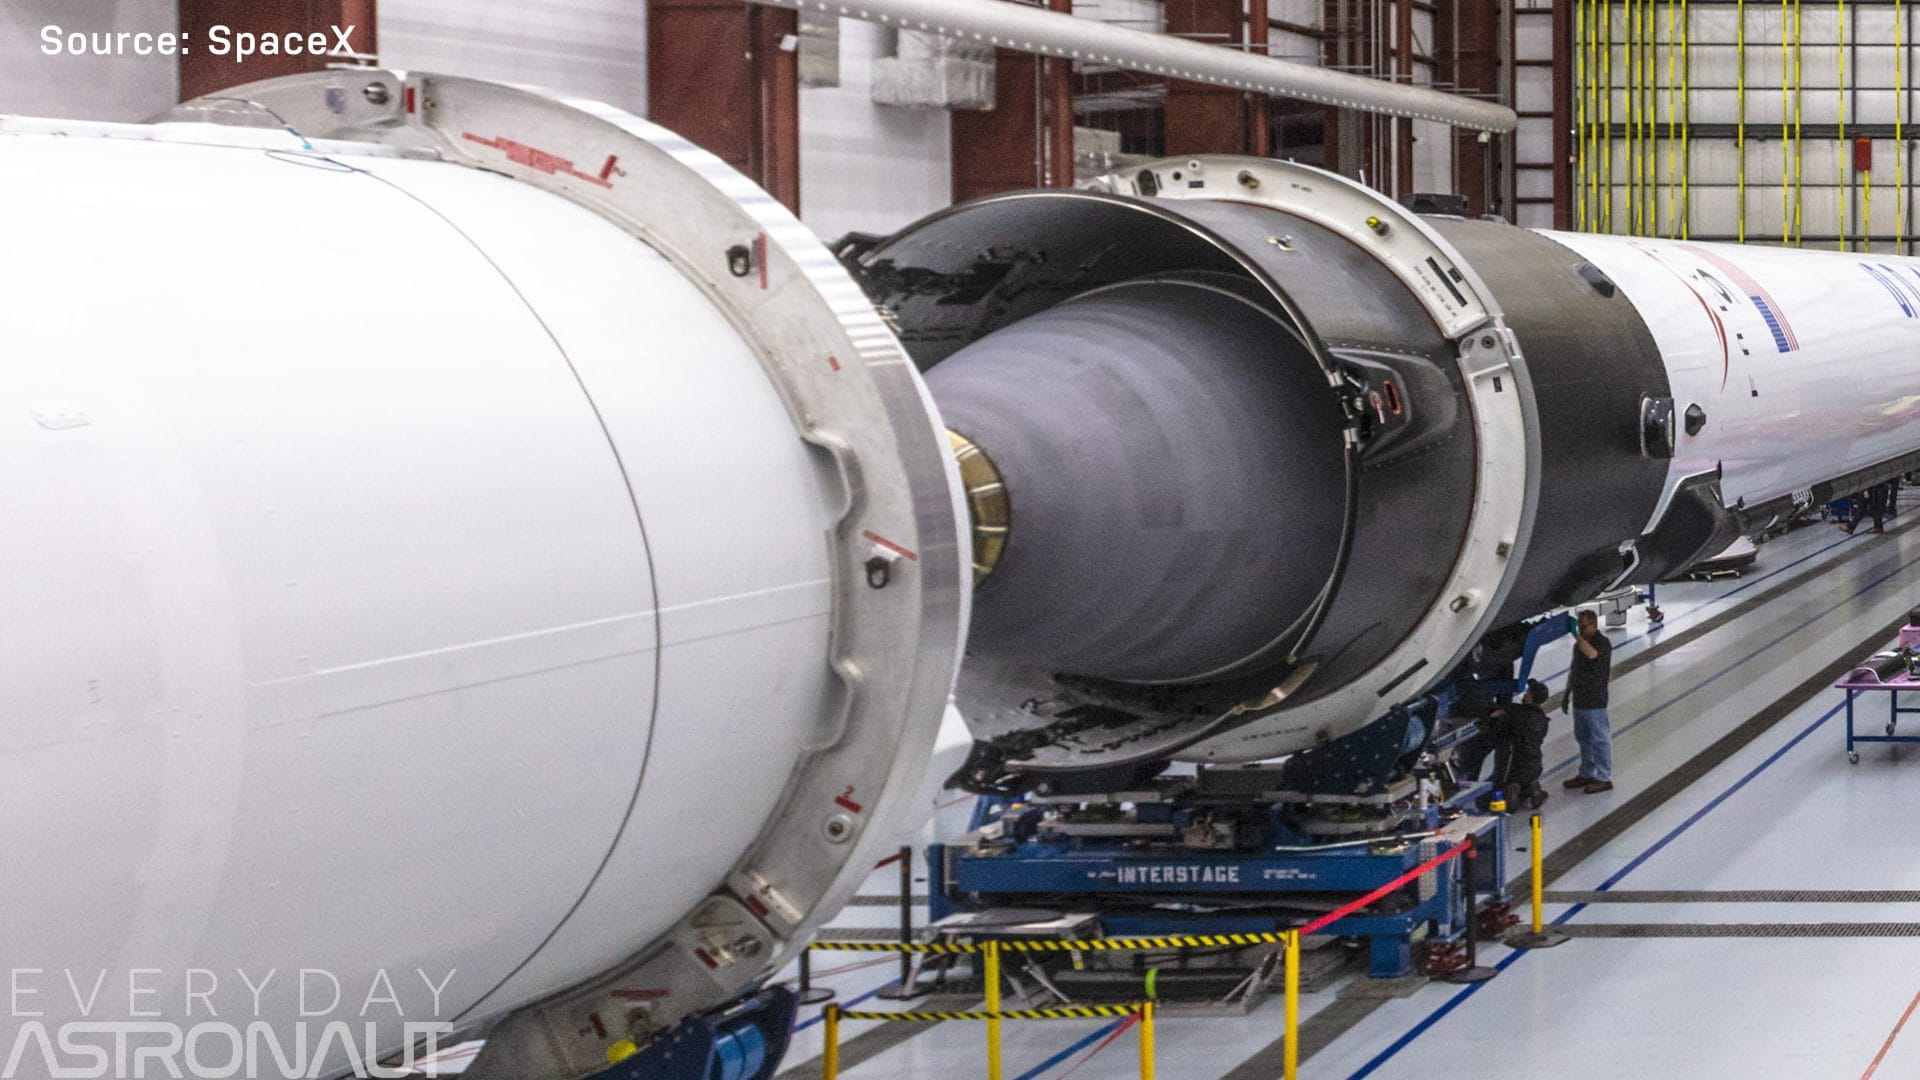
\includegraphics[width = 250px]{vacuumnozzle}
    \label{fig:vacuumnozzle}
    \caption{One Vacuum Engine on the Second Stage}
\end{figure}

So multistage rockets can be used to "switch" the nozzle type upon exiting the atmosphere for better performance in space. Another type of nozzle called the aerospike is a nozzle that can theoretically perform optimally in both atmospheric and vacuum conditions. Its design is such that its area of cross section changes dynamically with external pressure. It has its own drawbacks and as of today has not been used in an actual flight.

\newpage

\section{Re-entry Dynamics}
Getting space crafts to safely return back to Earth is certainly essential for manned vehicles, but the concept behind it is much more essential for futuristic inter-planetary travel ideas. The problem is that orbiting objects have extremely high kinetic energy per unit mass. This must obviously be reduced significantly as the craft approaches the Earths's surface. This can be done actively through using rocket engines, passively using the drag force of the atmosphere or a combination of the both. The drag reduces kinetic energy according to the equation $\Dot{T} = \mathbf{D} \cdot \mathbf{v}$. Considering the atmosphere to be exponential and flight hypersonic, the drag force can be given as: 
\[
	\mathbf{D} = - \frac{1}{2} C_d A V^2 \rho_0 e ^ {-H/H_0} \hat{\mathbf{v}}
\]

Plugging that in shows that the byproduct of drag is a tremendous amount of heat. Hence one of our constraints while making the re-entry trajectory is to minimise heat production. 

\subsection{Steep Ballistic Descent}

\begin{figure}[h!]
\centering
\begin{subfigure}{.5\textwidth}
  \centering
  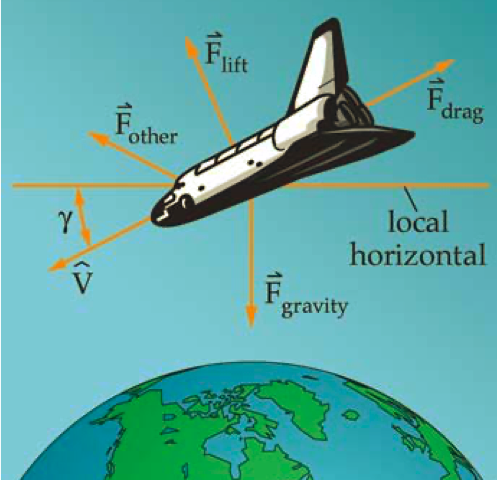
\includegraphics[width=150px]{entryForces}
  \caption{Forces applied on Re-entry}
  \label{fig:forces}
\end{subfigure}%
\begin{subfigure}{.5\textwidth}
  \centering
  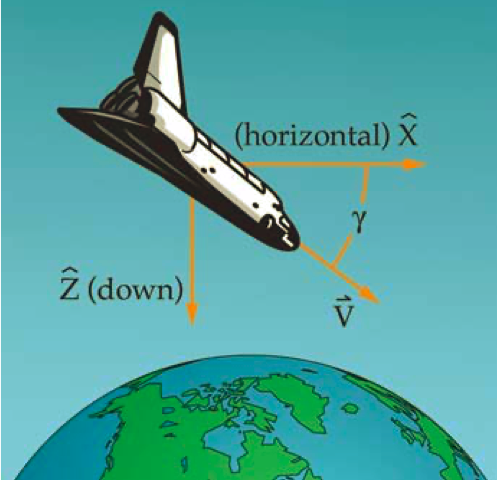
\includegraphics[width=150px]{entryFrame}
  \caption{Frame used for Equations}
  \label{fig:frame}
\end{subfigure}
\caption{Ballistic Re-entry}
\label{fig:entry}
\end{figure}

\newpage

We shall use the frame as shown in Figure \ref{fig:frame}. The equations are as follows:

\[
	\frac{dX}{dt} = V\: cos\:\gamma
\]
\[
	\frac{dH}{dt} = V \:sin\:\gamma
\]
\[
	m\frac{dV}{dt} = -D - mg \:sin\:\gamma
\]
\[
	mV\frac{d\gamma}{dt} = -mg\:cos\:\gamma
\]

Solving these equations by substituting above value of drag force. We assume we have a very steep angle of entry and that the angle changes very little over time. Also, the velocity can be assumed to be quite large for most part of the trajectory. This gives us:
\[
	T = \left[ B_0 + mgH_0 E_i(K_D \rho) \right]e ^{-K_D\rho}
\]
Where $E_i$ is the exponential integral function given by:
\[
	E_i(x) = \int_{-\infty}^{x} \frac{e^t}{t} dt
\]
And $K_d$ is given by:
\[
	K_D = -\frac{C_D A H_0}{m\: sin\: \gamma_i}
\]

We now endeavour to calculate the maximum acceleration experienced by the craft. This can be done by approximating the above function using the Taylor's Expansion and a few approximations. 
\[
	a_{max} = \frac{V_0^2 sin\:\gamma_i}{2H_0e}
\]

Plugging in a few values shows that this is not suitable for manned vehicles(upto 160g's!). Let's see what happens at a shallower angle of re-entry.

\subsection{Ballistic Re-entry}
We start out with the same equations but introducing centripetal acceleration as well.

\[
	\frac{dH}{dt} = V \:sin\:\gamma
\]
\[
	\frac{dV}{dt} = - \frac{1}{2} \frac{C_d A V^2}{m} \rho_0 e ^ {-H/H_0} - \left( g -\frac{V^2cos^2\gamma}{R_0 + H} \right) \:sin\:\gamma
\]
\[
	V\frac{d\gamma}{dt} = -\left( g -\frac{V^2cos^2\gamma}{R_0 + H} \right)\:cos\:\gamma
\]

Now for small angles, $cos\:\gamma \approx 1$ and $sin\:\gamma \approx \gamma$. Also, $H<<R_0$, the radius of the Earth. We can also neglect the small component of gravity compared to drag. Reducing above equations according to these approximations and solving via numerical techniques and mathematical approximations gives us the maximum deceleration under some general conditions as:
\[
	\frac{a_{max}}{g} \approx 8.3
\]
The maximum limit of the human body is around 8 times the acceleration due to gravity. The maximum deceleration is reduced by integrating lift or powered descent into the equation. By staying at higher altitudes for longer, the re-entry spans a longer duration but provides more "drag time" thereby reducing the maximum deceleration as well as reduces the heating rate of the craft. With the combination of lift and drag many techniques such as the \href{https://en.wikipedia.org/wiki/Boost-glide}{Skip Re-entry} have been devised for optimal re-entry. Re-entry isn't just a problem of getting objects back to Earth, getting objects like rovers to land on planets such as Mars is also a subset of this problem. Many interesting algorithms like the Polynomial Descent Gradient have been developed. An animation of the deployment of the rover Curiosity on Mars can be seen \href{https://www.youtube.com/watch?v=gwinFP8_qIM}{here}.

\subsection{Re-entry Corridor}
\begin{figure}[ht]
	\centering
    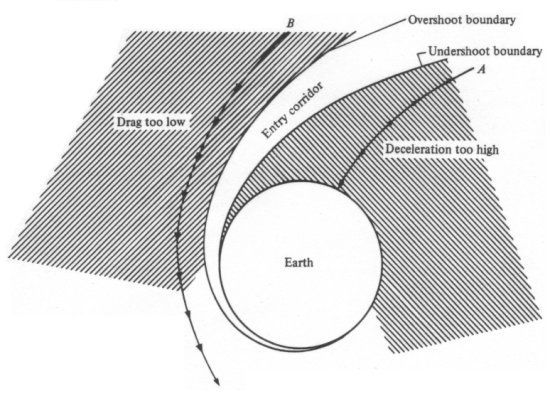
\includegraphics[width = 280px]{corridor}
    \label{fig:corridor}
    \caption{Re-entry Corridor}
\end{figure}

The re-entry corridor's upper boundary is defined by the boundary above which the vehicle risks "bouncing" off the atmosphere and back into space i.e. it is unable to slow down enough to be dragged down. The lower boundary is defined by conditions like maximum decelaration and maximum heating rate the craft can handle. These two depend on the initial entry angle $\gamma_i$ and the re-entry velocity as shown in the first subsection. These parameters along with the design are tweaked so that the corridor is such that the Guidance, Control and Navigation System(GNC) can safely carry the craft through the corridor. Below is a table that shows the tradeoff between the various quantities.

\begin{figure}[ht]
	\centering
    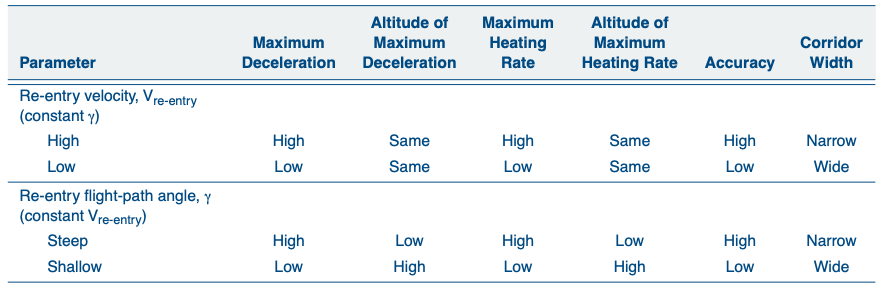
\includegraphics[width=\textwidth]{tradeoff}
    \label{fig:tradeoff}
    \caption{Tradeoff between re-entry parameters}
\end{figure}
 
 \newpage

\section{Mission Analysis}
\subsection{The Voyager Mission}
The Voyager mission was designed to take advantage of a rare geometric arrangement of the outer planetsz(once that comes every 176 years) in the late 1970s and the 1980s which allowed for a four-planet tour for a minimum of propellant and trip time. The Voyager 1 was launched on a shorter, faster trajectory on September 5, 1977 to allow  close flybys of Jupiter and its large moon Io, and Saturn and its large moon Titan. Voyager 2 was launched on August 20, 1977 and its trajectory was set to do a Jupiter and Saturn flyby and was later re-programmed to conduct flybys for Neptune and then further Uranus. After their respective flybys, both spacecrafts made their way past the heliosphere and into interstellar space where they continued to provide important scientific data. 

\begin{figure}[H]
	\centering
    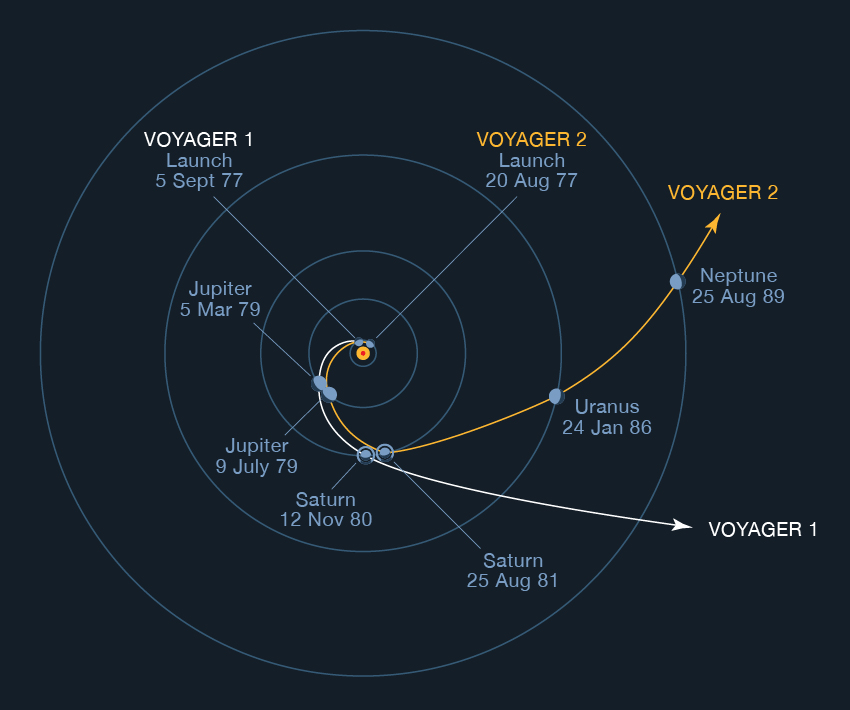
\includegraphics[height=300px]{voyager_trajectories}
    \label{fig:voyager_trajectories}
    \caption{Trajectories of the Voyager crafts}
\end{figure}

The crafts followed hyperbolic trajectories for the planetary flybys, details of the orbital elements can be found \href{https://voyager.jpl.nasa.gov/mission/science/hyperbolic-orbital-elements/}{here}. The Voyager mission was intended to be a five year mission but, it has been more than forty years and they crafts transmit useful data till date. This mission highlights the clever engineering for optimal use of planetary positions for achieving optimal use of resources. More information about the mission's current status is available \href{https://voyager.jpl.nasa.gov/mission/status/}{here}.

\subsection{Falcon 9's Landing}
The landing of the first stage of the Falcon 9 rocket by SpaceX back in 2011 was a great feat of engineering and a giant leap towards the reusability of rockets and commercial space travel. It involved a deep understanding of the topics discussed in this report and is an excellent example of the long road we have ahead of us in the journey of space exploration.\\
SpaceX was able to accomplish this feat with three primary sources of control:
\begin{itemize}
  \item Cold Gas Thrusters
  \item Grid Fins
  \item Thrust Vector Control
\end{itemize}

As we saw, aerodynamic forces do not act in space, hence the need for cold gas thrusters. These are nozzles positioned at the nose of the first stage that eject cold nitrogen to re-orient the stage and keep it positioned along the re-entry path. Upon entering the atmosphere, grid fins are deployed that take advantage of the atmospheric drag to keep the stage on track. This reduces the amount of fuel needed for landing. The engines primary job is to slow down the velocity of the stage down to zero but they are gimbaled to control roll, pitch and yaw for the final leg of the trajectory.

\begin{figure}[H]
	\centering
    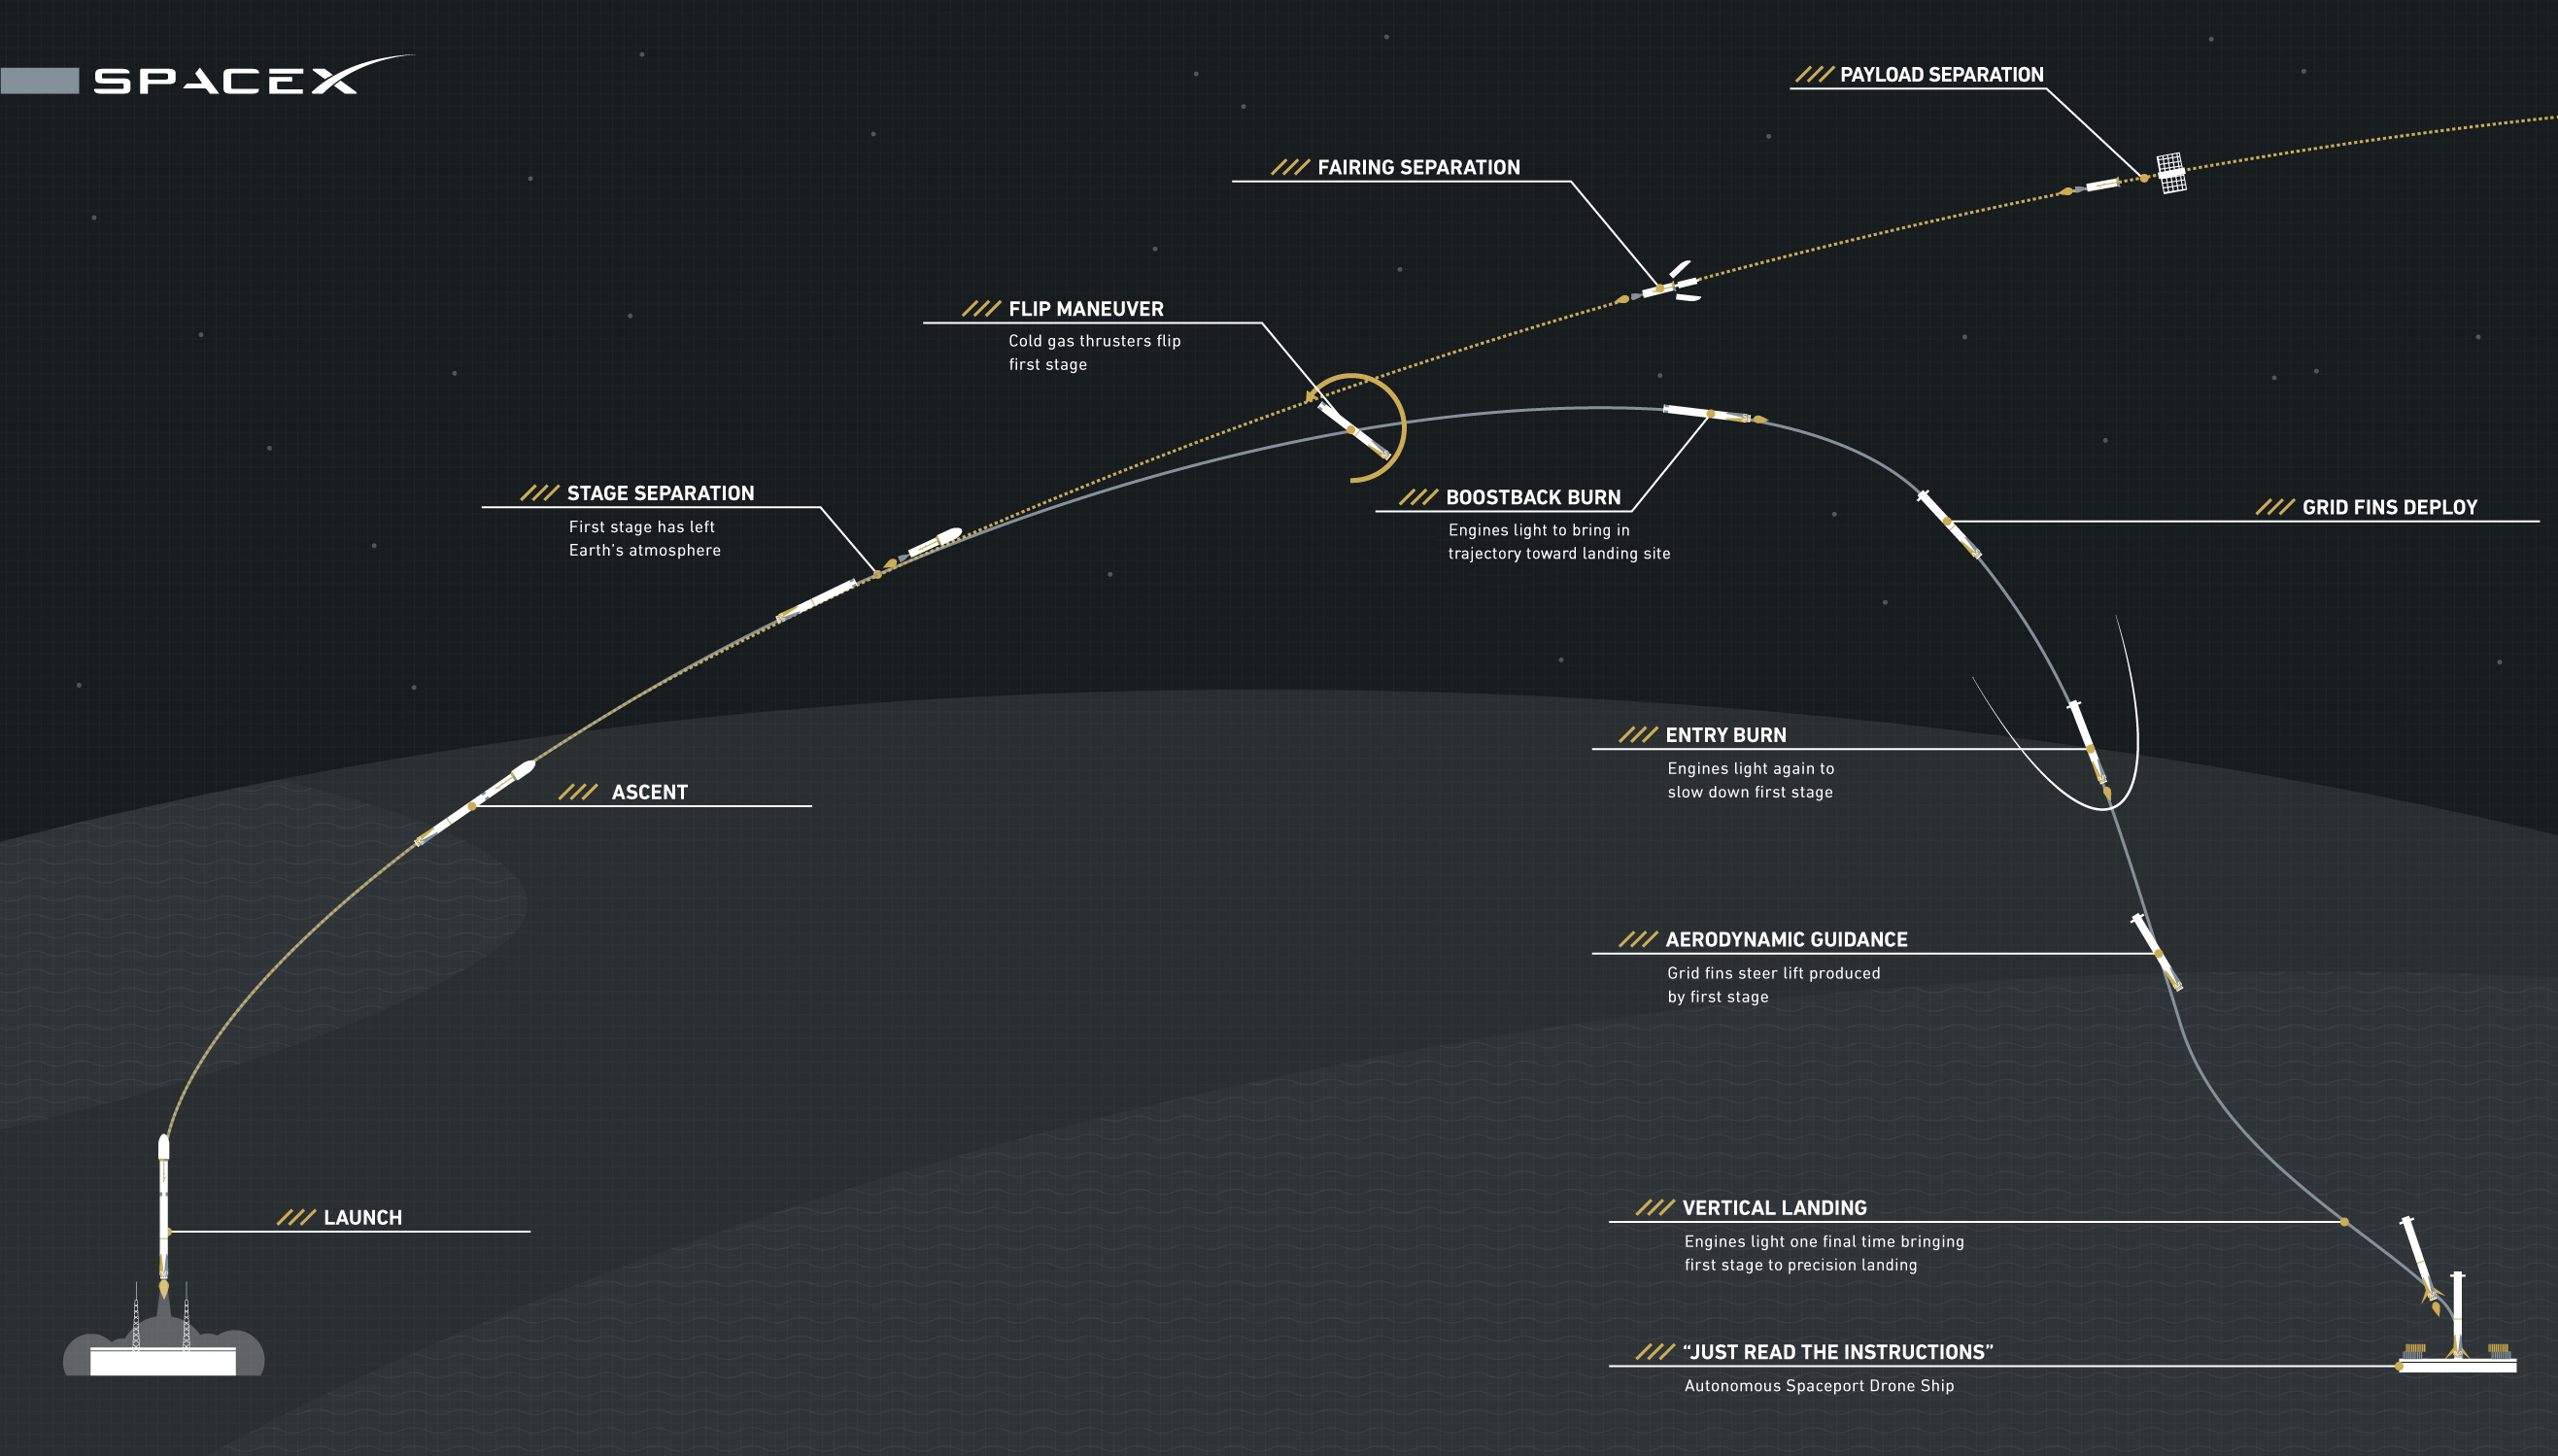
\includegraphics[height=200px]{Falcon_9_First_Stage_Reusability_Graphic}
    \label{fig:Falcon_9_First_Stage_Reusability_Graphic}
    \caption{Trajectory of the First and Second stages of the Falcon 9}
\end{figure}

\begin{figure}[H]
	\centering
    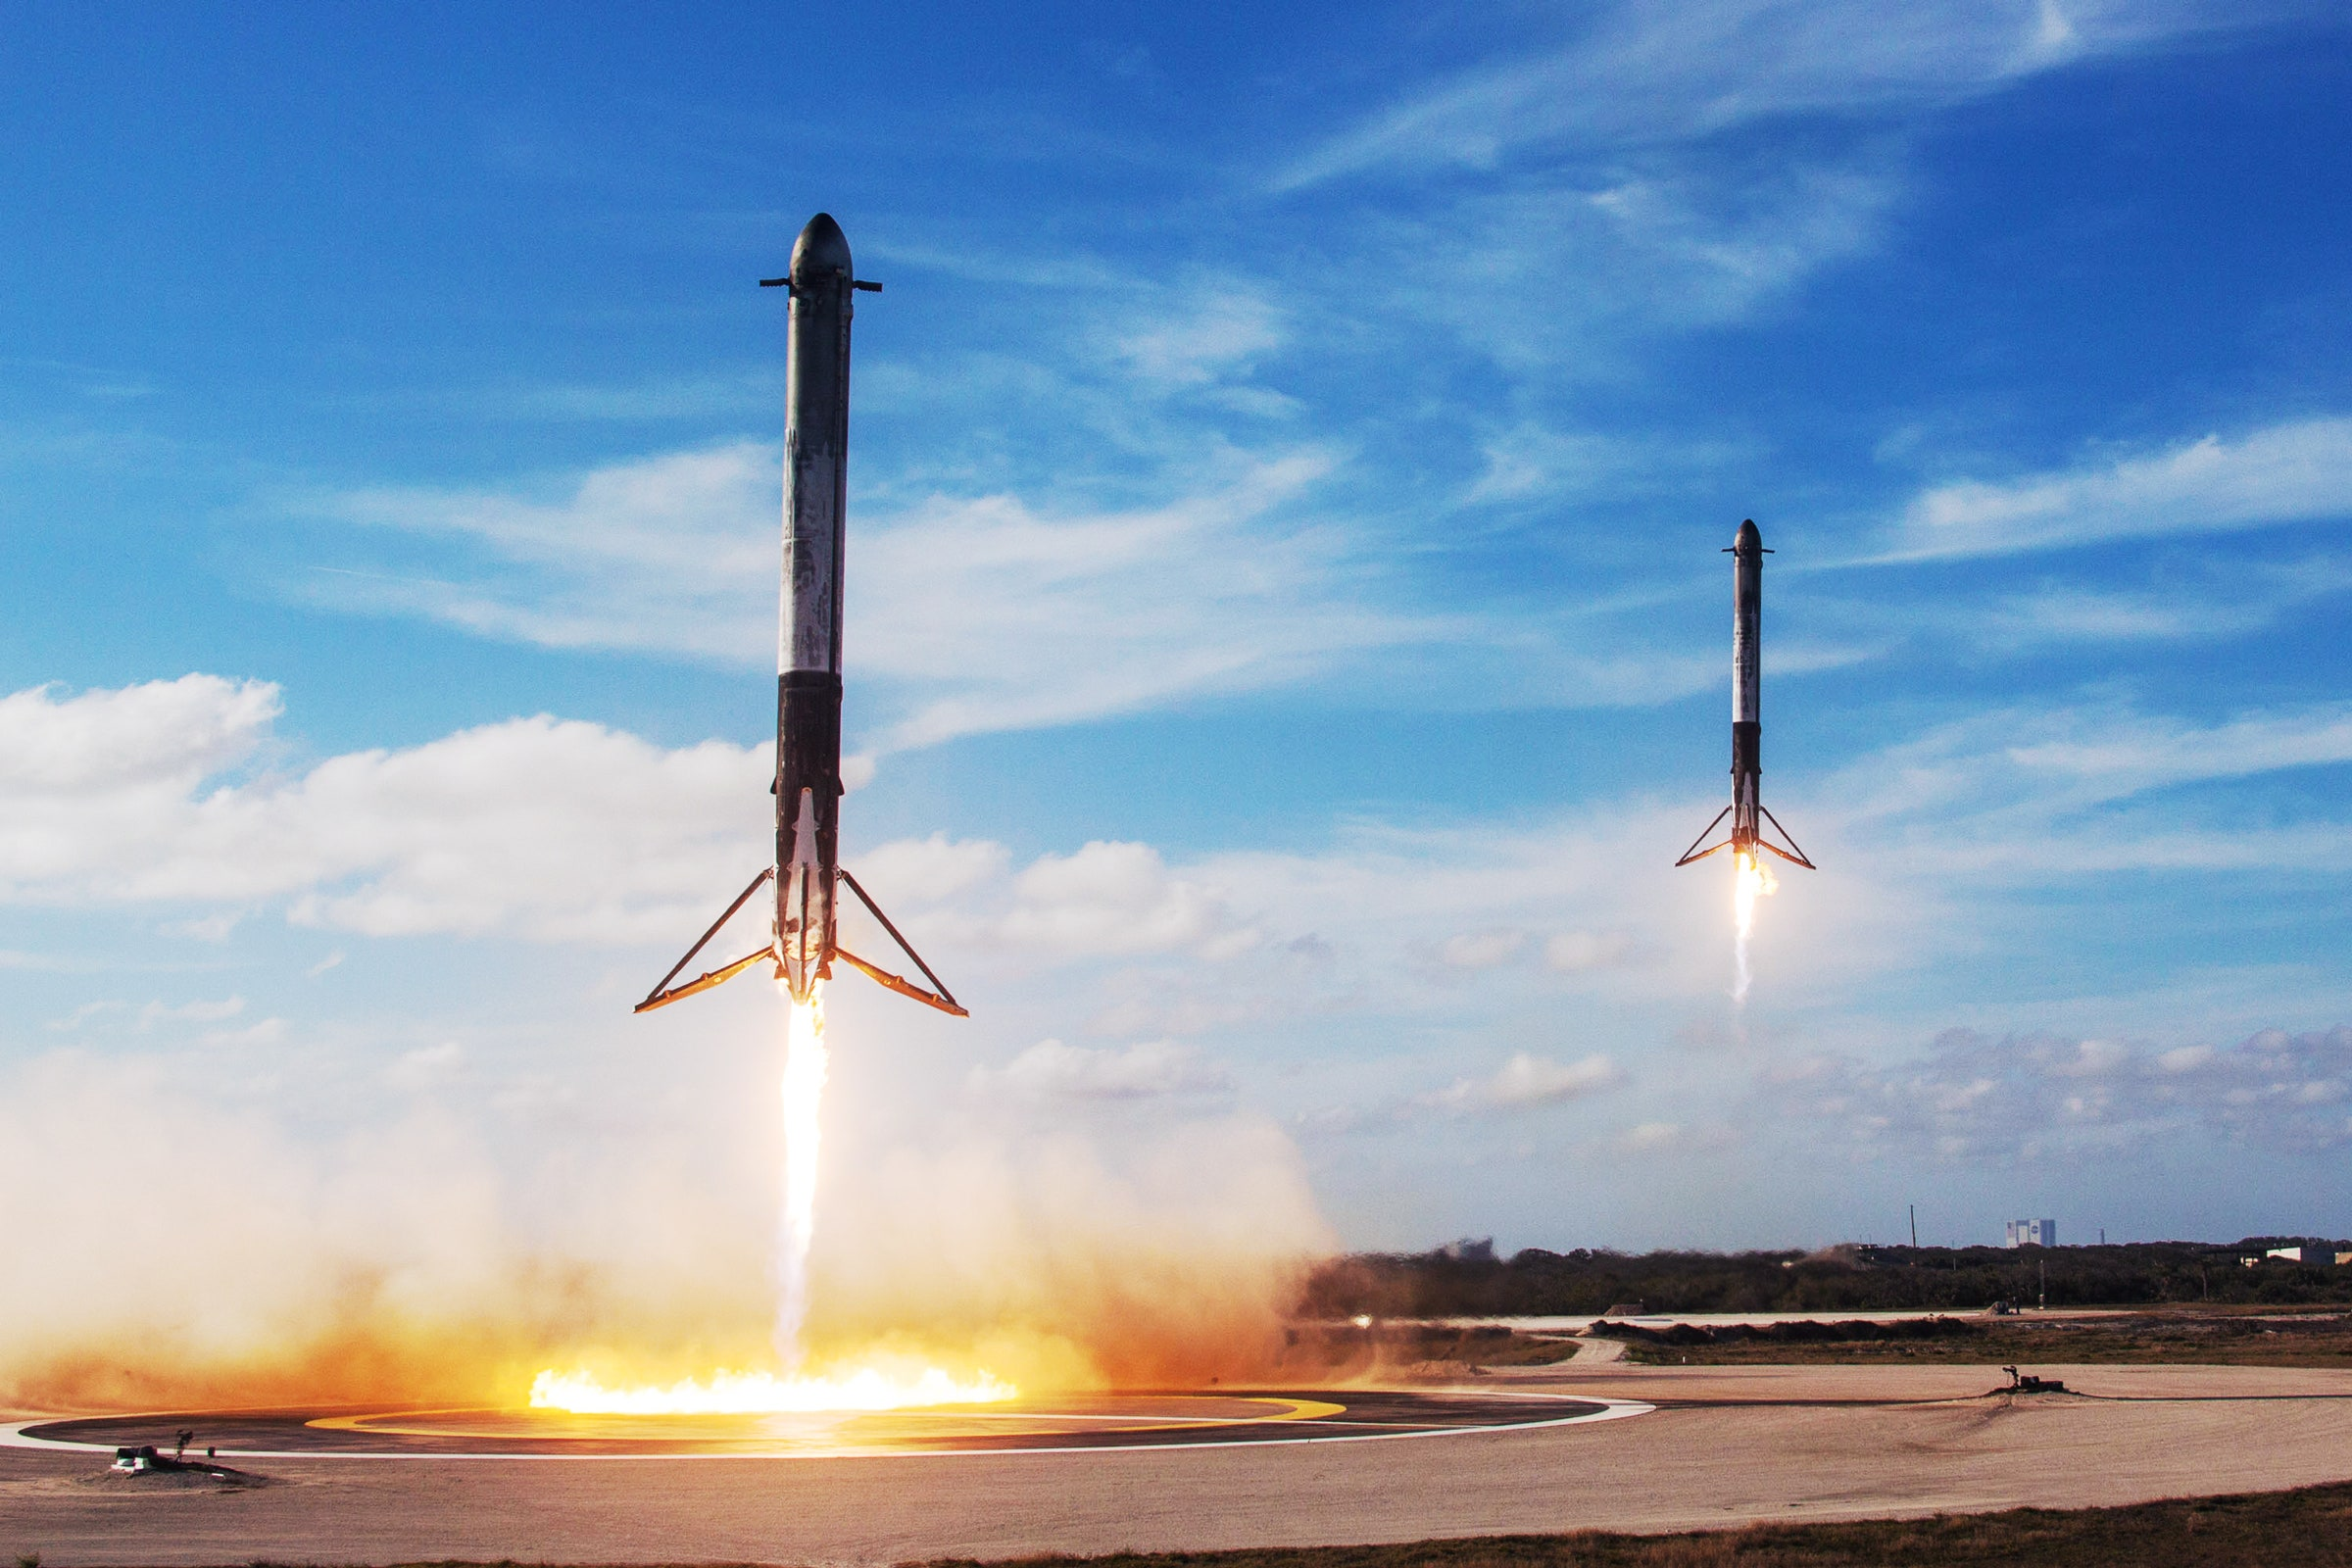
\includegraphics[height=200px]{spacexrocketreturn}
    \label{fig:spacexrocketreturn}
    \caption{Ground Landing of the boosters of the Falcon Heavy}
\end{figure}

I suppose anyone reading this report has watched a stage landing at one time or another, yet I include a \href{https://www.youtube.com/watch?v=sf4qRY3h_eo}{link} to one for the unfortunate who haven't. 

\newpage

\section{Bibliography}

Main material:\\
Spaceflight Dynamics - By : William E. Wiesel (Third Edition)\\
\vspace{1px}

Bell Engine:\\
\url{https://www.youtube.com/watch?v=D4SaofKCYwo&t=666s}\\
\vspace{1px}

Reentry material:\\
\url{https://www.faa.gov/about/office_org/headquarters_offices/avs/offices/aam/cami/library/online_libraries/aerospace_medicine/tutorial/media/iii.4.1.7_returning_from_space.pdf}\\
\vspace{1px}

Voyager Data:\\
\url{https://voyager.jpl.nasa.gov}\\
\vspace{1px}

SpaceX Data:\\
\url{https://cosmosmagazine.com/space/launch-land-repeat-reusable-rockets-explained}
\url{https://www.spacex.com}\\
\vspace{1px}

Some Other Material:\\
\url{https://www.nasa.gov}

\end{document}












